\section{Electric Fields in Matter} % (fold)
\label{sec:Electric Fields in Matter}

\subsection{Polarization} % (fold)
\label{sub:Polarization}

\begin{frame}
  \frametitle{Dielectrics}

  In most everday objects belong to one of two larges classes:
  \begin{itemize}

      \item \textbf{Conductors}: charges aree free to move about through the material, not associated twith any particular nucleus but roam around at will

      \item \textbf{Dielectrics (Insulators)}: All charges are attached to specific atoms or molecules, all they can do is move a bit within the atom or molecule.

  \end{itemize}

  Two principal mechanisms: Electric fields can distort the charge distribution of a dielectric atom or molecule: \textit{stretching} and \textit{rotating}.



\end{frame}

\begin{frame}
  \frametitle{Induced Dipoles}

  What happens to a neutral atom when it is placed in electric field $\overrightarrow{E}$ ?

  \begin{itemize}

      \item Although the atom as a whole is electrically neutral, there is a positively charged core (the nucleus) and a negatively charged electron.
      \item The nucleus is pushed in the direction of the field, and the electrons the opposite way.

  \end{itemize}

  The atom is \textbf{polarized}, with a tiny \textbf{dipole moment} $\overrightarrow{p}$, which points in the same direction as $\overrightarrow{E}$, proportional to the field:
  \begin{equation}
    \overrightarrow{p} = \alpha \overrightarrow{E}
  \end{equation}

  where $\alpha$ is called \textbf{atomic polarizability}.



\end{frame}

\begin{frame}
  \frametitle{Induced Dipoles}

  For some neutral molecules like carbon dioxide, they frequently polarize more readily in some directions than in others, for example:
  \begin{equation}
    \overrightarrow{p} = \alpha_\perp \overrightarrow{E}_\perp + \alpha_\parallel \overrightarrow{E}_\parallel
  \end{equation}

  For a completely asymmetrical molecule, there is the most general linear relationship between $\overrightarrow{E}$ and $\overrightarrow{p}$:
  \begin{equation}
    \begin{cases}
      p_x = \alpha _{xx} E_x + \alpha _{xy} E_y + \alpha_{xz} E_z \\
      p_y = \alpha _{yx} E_x + \alpha _{yy} E_y + \alpha_{zz} E_z \\
      p_z = \alpha _{zx} E_x + \alpha _{zy} E_y + \alpha_{zz} E_z 
    \end{cases}
  \end{equation}

  The induced dipole moment may not be in the same direction as $\overrightarrow{E}$.

\end{frame}

\begin{frame}
  \frametitle{Alignment of polar molecules}


  For some molecules which have built-in, permanent dipole moments, called \textbf{polar molecules}, e.g. water molecule, 
  \begin{itemize}

      \item If the champ is uniform, the force on the positive end exactly cancels the force on the negative end. However, there will be a torique
        \begin{align}
          \overrightarrow{N} &= \overrightarrow{F}_- \overrightarrow{r}_- + \overrightarrow{F}_+  \overrightarrow{r}_+ 
                             = \frac{\overrightarrow{d}}{2} \times q \overrightarrow{E} - \frac{\overrightarrow{d}}{2} \times (-q \overrightarrow{E}) = q \overrightarrow{d} \times \overrightarrow{E} \\
                             &= q \overrightarrow{d} \times \overrightarrow{E} = \overrightarrow{p} \times \overrightarrow{E} 
                            = \displaystyle\frac{1}{4 \pi \epsilon_0} 
        \end{align}




  \end{itemize}

\end{frame}

\begin{frame}
  \frametitle{Alignment of molecules and polar molecules}



  \begin{itemize}

      \item If the champ is not uniform, $\overrightarrow{F}_+$ does not balance $\overrightarrow{F}_+$, there will be a net force on the dipole:
        \begin{equation}
          \overrightarrow{F} = \overrightarrow{F}_+ + \overrightarrow{F}_- = q(\overrightarrow{E}_+ - \overrightarrow{E}_-) = q(\Delta \overrightarrow{E})
        \end{equation}

  Assuming the dipole is very short, we approximate the small change in the electric field:

  \begin{equation}
    \Delta E_x = \nabla E_x . \overrightarrow{d},\quad \Delta \overrightarrow{E} = (\overrightarrow{d}. \nabla) \overrightarrow{E}
  \end{equation}

  and therefore 
  \begin{equation}
    \overrightarrow{F} = (\overrightarrow{p}.\nabla)\overrightarrow{E}
  \end{equation}



  \end{itemize}

  The torque about the center of the dipole in a nonuniform field is:
  \begin{equation}
    \overrightarrow{N} = \overrightarrow{p} \times \overrightarrow{E} + \overrightarrow{r} \times \overrightarrow{F}
  \end{equation}

\end{frame}
\begin{frame}
  \frametitle{Polarization - Conclusion}

  The result of placing a piece of dielectric material in an electric field is that the material becomes \textbf{polarized}, i.e. pointing along the direction of the field, either a tiny dipole moment is induced for neutral atoms, or a torque for polar molecules.

  A measure for this effect is 
  \begin{equation}
    \overrightarrow{P} = \text{dipole moment per unit volume}
  \end{equation}

  which is called \textbf{polarization}.

\end{frame}
% subsection Polarization (end)

\subsection{The field of a polarized object} % (fold)
\label{sub:The field of a polarized object}

\begin{frame}
  \frametitle{Bound Charges}

  Suppose we have a piece of polaried material, i.e. a lot of microscopic dipoles \textit{lined up}. Given $\overrightarrow{P}(\underline{\overrightarrow{r}})$, what is the field produced by this object (i.e. caused by the polarization)? 

  \begin{figure}[H] %h:当前位置, t:顶部, b:底部, p:浮动页
    \centering
    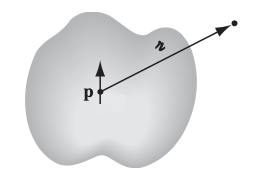
\includegraphics[width=0.4\textwidth]{./assets/Bound-charges.png}
  \end{figure}
  
\end{frame}

\begin{frame}
  \frametitle{Bound Charges}

  It is easier to work with the potentiel. 

  For a single dipole $\overrightarrow{p}$, 
  \begin{equation}
    V(\overrightarrow{r}) = \displaystyle\frac{1}{4 \pi \varepsilon_0} \displaystyle\frac{ \overrightarrow{p} . \widehat{\overrightarrow{\underline{{r}}}}}{\underline{r}^{2}}
  \end{equation}

  The total potential is the integration of each volume element, whose dipole moment $\overrightarrow{p} = \overrightarrow{P} \mathrm{d} \tau'$

  \begin{align}
    V &= \displaystyle\frac{1}{4 \pi \epsilon_0} \int_{V}^{} \displaystyle\frac{\overrightarrow{P}(\overrightarrow{r}'). \widehat{\overrightarrow{\underline{r}}}}{\underline{r}^2} \mathrm{d} \tau' \\
      &= \displaystyle\frac{1}{4 \pi \epsilon_0} \int_{V}^{} \overrightarrow{P}. \nabla ' 
  \end{align}

  
\end{frame}

% subsection The field of a polarized object (end)
